% TEX program=xelatex
\documentclass[10pt,twocolumn,letterpaper]{article}

\usepackage{cvpr}
\usepackage{times}
\usepackage{epsfig}
\usepackage{graphicx}
\usepackage{amsmath}
\usepackage{amssymb}
\usepackage{enumitem}
\usepackage{subcaption}
\usepackage{float}

% Include other packages here, before hyperref.

% If you comment hyperref and then uncomment it, you should delete
% egpaper.aux before re-running latex.  (Or just hit 'q' on the first latex
% run, let it finish, and you should be clear).
\usepackage[breaklinks=true,bookmarks=false]{hyperref}
\cvprfinalcopy % *** Uncomment this line for the final submission

\def\httilde{\mbox{\tt\raisebox{-.5ex}{\symbol{126}}}}

\graphicspath{ {./figures/} }


% Pages are numbered in submission mode, and unnumbered in camera-ready
%\ifcvprfinal\pagestyle{empty}\fi
\setcounter{page}{1}
\begin{document}

%%%%%%%%% TITLE
\title{Generating Anime Avatars Using Generative Adversarial Networks \\
\large Final Report for Deep Learning Course}

\author{Wang Ao\\
Tsinghua University\\
2017010395\\
{\tt\small wa17@mails.tsinghua.edu.cn}
% For a paper whose authors are all at the same institution,
% omit the following lines up until the closing ``}''.
% Additional authors and addresses can be added with ``\and'',
% just like the second author.
% To save space, use either the email address or home page, not both
\and
Sun Ziping\\
Tsinghua University\\
2015013249\\
{\tt\small me@szp.io}
\and
Cui Yanfei\\
Tsinghua University\\
2017012326\\
{\tt\small 929881841@qq.com}
}

\maketitle
%\thispagestyle{empty}

%%%%%%%%% ABSTRACT
\begin{abstract}
% Goal, Approach, Novel Contribution, Conclusion
In the past few years, computer vision has achieved rapid development, and
Generative Adverarial Networks~\cite{GAN} have attracted wide attention since
proposed in 2014. In this paper, we aimed to generate from noise and to transfer
from existing pictures to anime avatars, which is an interesting and practical
task. There have been many paper achieving this kind of task, such as
DCGAN~\cite{DCGAN}, CycleGAN~\cite{CycleGAN2017} and
CartoonGAN~\cite{CartoonGAN}. In this paper, we reimplement these three models
and tune them to achieve better performance on this specific task. And then, we
give several novel loss functions to make models perform better, such as face
landmark loss. At last, we compare the different results between these three
models and come to the conclusion that DCGAN is generally a good choice to
generate images from noise, CycleGan performs the best on image tansfering while
CartoonGAN tends to preserve image details, which results to a poorer
performance.
\end{abstract}

%%%%%%%%% BODY TEXT
\section{Introduction}

% GAN, DCGAN, CycleGAN, Evalutaion method
Generally speaking, image generating and style transferring belongs to the
generative problem. And deep generative models have achieved impressive success
in this field. Among all deep generative models, the most outstanding ones, for
the time being, are Generative Adversarial Networks (GANs) and Variational
Autoencoders (VAEs). In our work, we focus on GANs.

Traditional GANs consist of two parts, the generator and the discriminator. The
generator tries to generate fake outputs similar to the real data, while the
discriminator tries to tell the real ones apart from the fake ones. When they
trained together, the discriminator drives the generator to generate realer
outputs, and meanwhile, the generated realer outputs also drive the
descriminator to jugde more correctly. And finally, in order to deceive the
discriminator, the generator can be well-trained for the generating task, that's
exactly what we want. It is also notable that these two parts may not
necessarily be trained exactly simultaneously. One part can be pretrained, or
they can be trained alternatively.

As mentioned above, there are two ways to generate anime avatars:

\begin{itemize}[noitemsep, topsep=0pt]
   \item directly generate a anime avatar from random noise
   \item generate corresponding anime avatar from real human avatar
\end{itemize}

For the first approach, DCGAN is among one of the most state-of-the-art models.
It is a variation of GAN, in which transposed convolutions are added. It is
mainly aimed for image generating tasks. Transposed convolutions are the inverse
operation of normal convolutions, and they broadcast input values through the
kernels, resulting a larger output shape, which is useful for up-sampling.

As for the second approach, according to the dataset given, it can be classified
to two kinds of problems. One is based on paired image transfer, while the other
is unpaired. In our work, dataset is unpaired. CycleGANs perform best on this
task. CycleGAN consists of two generators and two descriminators. Source images
first goes through one generator resulting in fake target images and then goes
through the other generator producing reconstruction source images. And for the
target images, they are processed in a similar way. The origin and
reconstruction images can be compared to get a cylce consistency loss, which
helps the model to be trained.

We also take a look at CartoonGAN. It is suitable for image transferring but
without a cyclic structure. Two novel losses are proposed: (1) a semantic
content loss, which forces the features of photos and cartoons to be close, and
(2) an edge-promoting loss to preserve clear edges, since edges in cartoons are
generally clearer than that of photos.

However, it still remains to be a difficult question how to evaluate the
performance of a generative model. So we just manually analyze the generated
images. Though this accessment method is subjective, the result is generally
universal.

%------------------------------------------------------------------------
\section{Related Work}

\subsection{Non-photorealistic rendering (NPR)}
In order to mimic specific artistic styles (including
animation~\cite{rosin2012image}), many automatic and semi-automatic NPR
algorithms have been developed. Most of the works are animated by using a simple
shadow rendering method~\cite{saito1990comprehensible}. One technique, called
\textsl{cel shading}, is widely used in the creation of games, animations, and
movies, saving artists a lot of time~\cite{luque2012cel}.

To mimic the cartoon style, people have developed various methods to create
images with flat shadows. These methods either use image
filtering~\cite{winnemoller2006real} or use specific transformation
formulas~\cite{xu2011image} in optimization problems. However, it is difficult
to capture rich artistic styles using only simple mathematical formulas. In
particular, filtering or optimizing the entire image does not create the
high-level abstractions that artists typically require. For portraits, people
also have special algorithms~\cite{yang2010semantics, rosin2015non}, in which
semantic segmentation can be automatically derived by detecting facial
components. However, these methods cannot handle general images.

\subsection{Convolutional neural networks}
With the great success of convolutional neural networks
~\cite{krizhevsky2012imagenet, lawrence1997face} in the field of computer
vision, people are looking forward to their performance in the field of image
style transfer and image generation. Compared with the traditional complex NPR
algorithm~\cite{saito1990comprehensible,luque2012cel}, CNN is indeed more
convenient and more applicable. For example, in the task of image style
transfer, the VGG network~\cite{VGG} has a good ability to extract picture
features.

For the style and content of the image, Gatys et al.~\cite{NST} first proposed a
CNN-based neural style transfer (NST) method that can transfer the style of a
picture from one picture to another. They use a feature map of a pre-trained VGG
network to extract picture content and optimize the resulting image, so that it
can match the corresponding texture information described by the global Gram
matrix~\cite{gatys2015texture} while retaining the original content of the
image. However, such operations caused a serious loss of the edge information
and shadow information of the picture.

\subsection{Image synthesis with GANs}
The other method using GANs~\cite{GAN} has achieved great imporvement.
It has achieved the state of the art results in the fields of text-to-image
translation~\cite{reed2016generative}, image inpainting~\cite{yeh2016semantic},
and image super-resolution~\cite{ledig2017photo}, etc. The key idea of the GAN
model is to train two networks (generator and discriminator). Iteratively, the
adversarial loss provided by the discriminator transforms the generated image
into a target manifold~\cite{yeh2016semantic}.

Some literatures~\cite{dumoulin2016adversarially,isola2017image,
karacan2016learning} provided solutions using GANs for pixel-level image
synthesis problems. However, these methods require paired data sets during the
training process, but such high-quality data sets are difficult to obtain and
therefore cannot be used for our training.

%------------------------------------------------------------------------
\section{Approach}

\subsection{Prepare Dataset}

We downloaded three datasets. One is real person photos, and the other two
belongs to anime avatars. The datasets are show in Table \ref{tab:datasets}, and
some examples drawn from datasets are show in Figure \ref{fig:dataset-examples}.

\begin{table}[h]
   \centering
   \begin{tabular}{|c|c|c|}
   \hline
   name & category & no of samples \\ \hline
   Anime & labeled anime avatars & 115087 \\ \hline
   Thumbs & unlabeled real photos & 3666 \\ \hline
   Faces & unlabeled anime avatars & 51223 \\ \hline
   \end{tabular}
   \caption{The dataset we use in our project. We will refer to these dataset
   using their name in this paper.}
   \label{tab:datasets}
\end{table}

\vspace{-2.5em}
\begin{figure}[h]
   \centering
   \begin{subfigure}{0.48\linewidth}
      \centering
      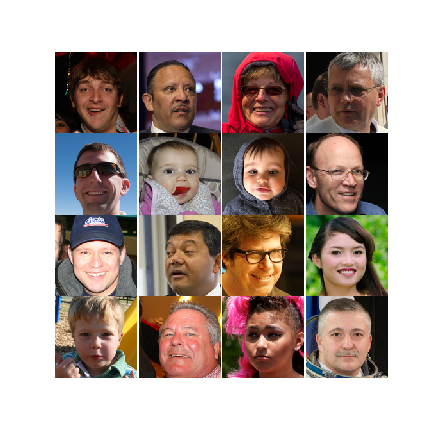
\includegraphics[width=\linewidth]{thumbs-examples}
      \vspace{-2em}
      \caption{Examples from Thumbs}
   \end{subfigure}
   \begin{subfigure}{0.48\linewidth}
      \centering
      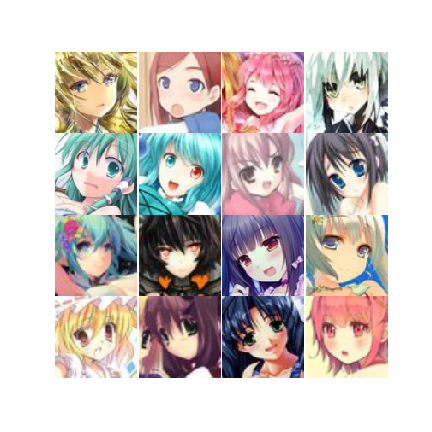
\includegraphics[width=\linewidth]{faces-examples}
      \vspace{-2em}
      \caption{Examples from Faces}
   \end{subfigure}
   \caption{Some example images from datasets}
   \label{fig:dataset-examples}
\end{figure}

\subsection{Generate from Noise Using DCGAN}

\begin{figure}[t]
   \centering
   \begin{subfigure}{\linewidth}
      \centering
      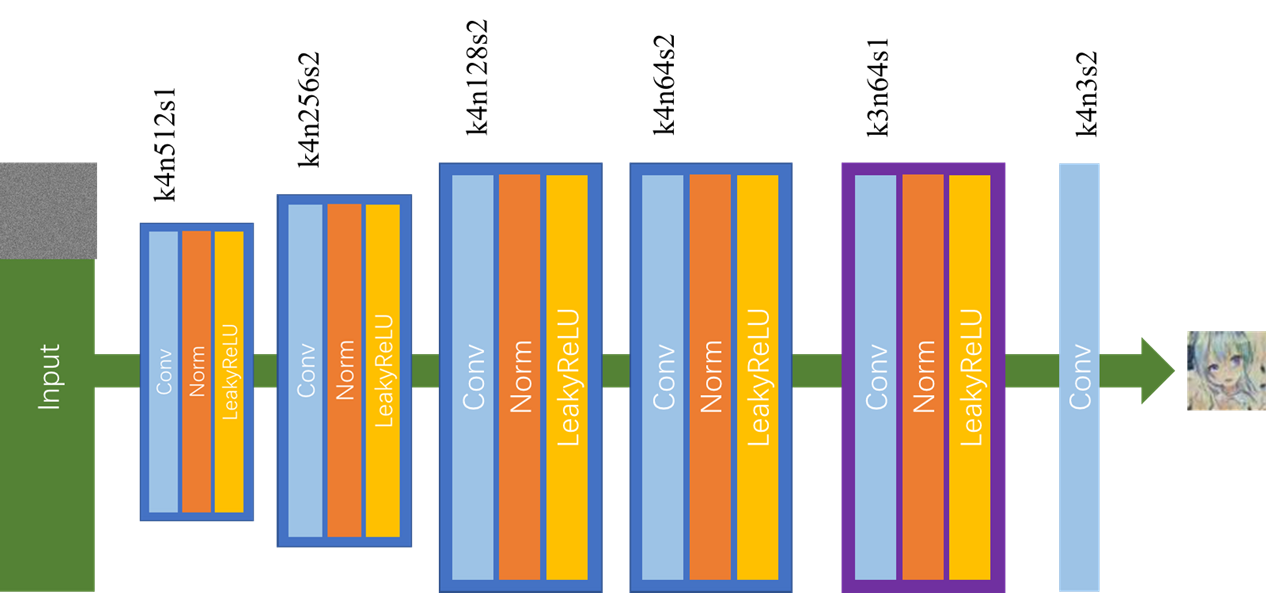
\includegraphics[width=.7\linewidth]{dcgan-g}
      \caption{Generator Architecture of DCGAN}
   \end{subfigure}
   \begin{subfigure}{\linewidth}
      \centering
      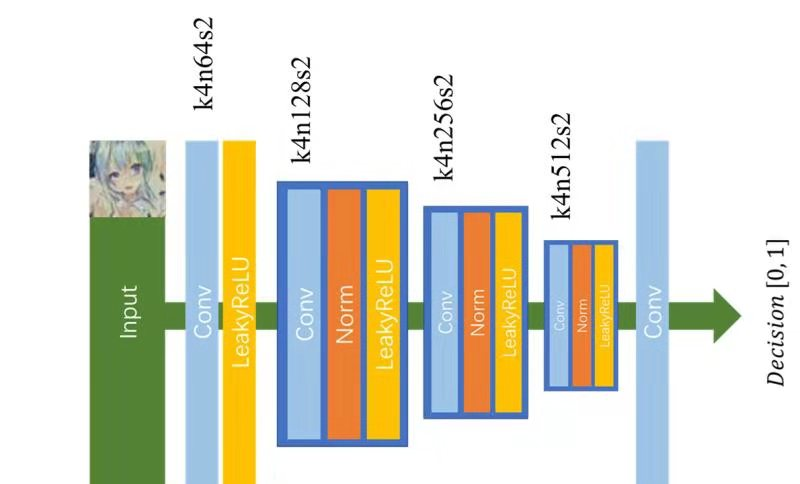
\includegraphics[width=.7\linewidth]{dcgan-d}
      \caption{Discriminator Architecture of DCGAN}
   \end{subfigure}
   \caption{Architecture of DCGAN. Here the number of k represents kernel size,
   n is the output size and s is stride}
   \label{fig:dcgan-arch}
\end{figure}

The architecture of our DCGAN model is shown in Figure \ref{fig:dcgan-arch}. The
input of the generator is a noise of length 100 drawn from normal standard
normal distribution. Then the input is expanded to the shape of
$512\times 4\times 4$ and goes through another 3 transposed convolution layer
up-sampling to the shape of $64\times 32\times 32$, each of which reduce the
input channels to half and expand the input size twice. And then the input is
processed by a size-preserving convolution layer called extra layers by us,
which changes the channel number to 3. Finally the input goes thought a
transposed convolution layer, which doubles the size. Every convolution layer
except the last one is followed by a batch normalization layer and a leakly ReLU
activiation layer. The last convolution layers outputs directly to the Tanh
activiation layer. Thus, the generated image has a size of
$3\times 64\times 64$, of which elements are in range $(-1, 1)$.

The discriminator is like a reverse version of the generator. The input size is
$3\times 64\times 64$, it is first converted to the size of
$64\times 32\times 32$ by a convolution layer. And then it undergoes 3
convolution layers, each of which doubles the channel number and cut the size to
half. Then it goes through a channel-and-size-preserving convolution layer, and
the output is of size $512\times 4\times 4$. Finally, the data is processed by
one convolution layer, of which the output is of size $1\times 1\times 1$. It is
notable that the descriminator does not use any fully connected layer.

We use Anime dataset as the input of DCGAN. The input is normalized to standard
normalization distribution, because the fake images also obey this distribution.
The training procedure consists of two phases. In the first phase, the generated
fake images and the real images are feed to discriminator and measured with
binary cross entropy (BCE) loss. In the second phase, the loss function tries the make
the generator generate images that trick the descriminator into thinking they
are real.

\subsection{Transfer from Real Photos Using CycleGAN}

\begin{figure*}[h]
   \centering
   \begin{subfigure}{.32\linewidth}
      \centering
      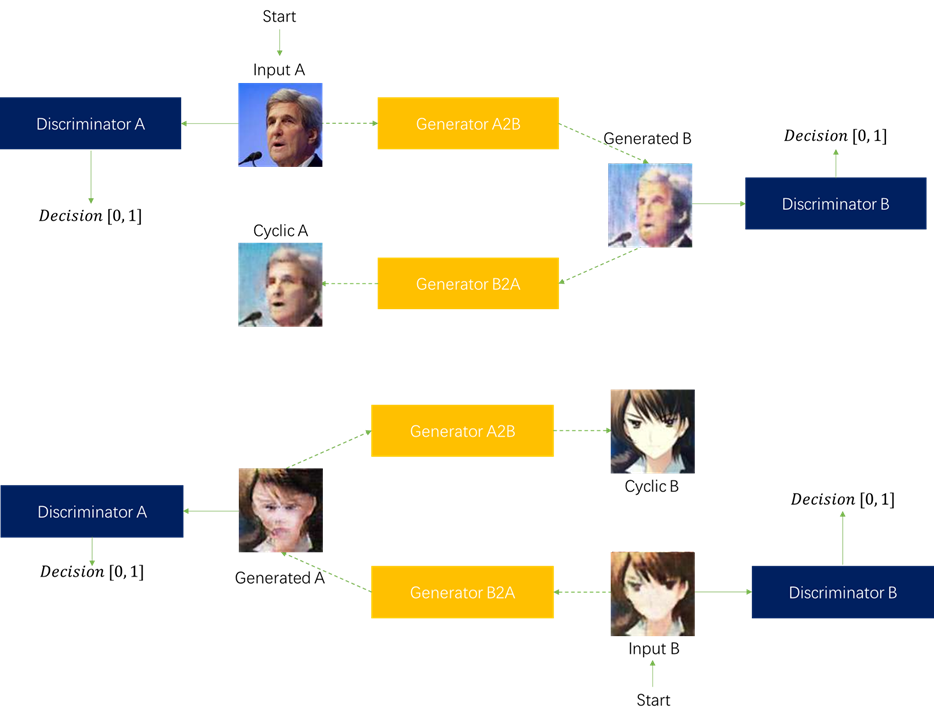
\includegraphics[width=.9\linewidth]{cyclegan-arch}
      \caption{Whole Architecture of CycleGAN}
   \end{subfigure}
   \begin{subfigure}{.32\linewidth}
      \centering
      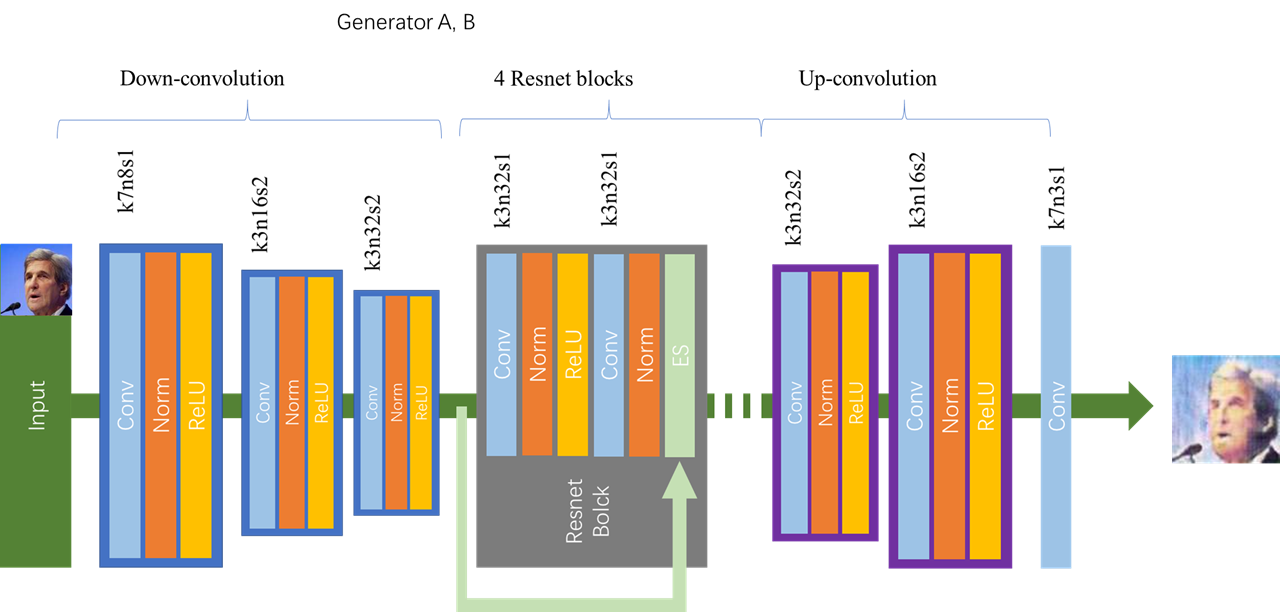
\includegraphics[width=.9\linewidth]{cyclegan-g}
      \caption{Generator of CycleGAN}
   \end{subfigure}
   \begin{subfigure}{.32\linewidth}
      \centering
      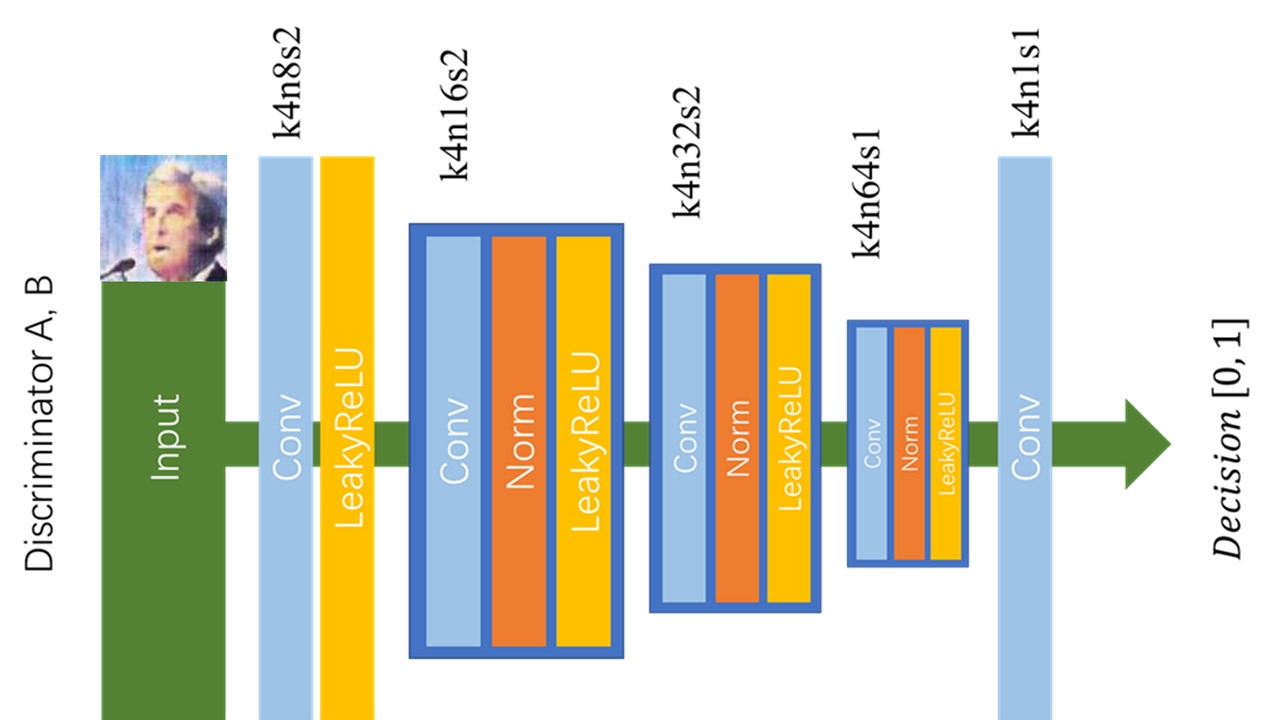
\includegraphics[width=.9\linewidth]{cyclegan-d}
      \caption{Discriminator of CycleGAN}
   \end{subfigure}
   \caption{Architecture of CycleGAN}
   \label{fig:cyclegan-arch}
\end{figure*}

Figure \ref{fig:cyclegan-arch} shows the architecture of out CycleGAN. CycleGAN
consists of two generators and two discriminators. The generators use two
down-sampling convolution layers, 4 ResNet blocks and two up-sampling
convolution layers. Since the model is a bit too large to fit in our computer's
GPU memory, the number of channels is made smaller than DCGAN. At first, we use
one down-sampling and one up-sampling, but preliminary experiment show that
shallower down-sampling and up-sampling layers lead to poorer generization
ability of the networks. So we change the numbers of down-sampling and
up-sampling layers to two. And it seems the networks work much more better.

The discriminators are similar to the ones of DCGAN. But the outputs contain
not only one element. The discriminators are binary classification models, so
the output shapes do not matter, as the real labels and fake labels can be any
shape of ones and zeros.

We use Thumbs dataset and Faces dataset as the input of CycleGAN. Hereinafter,
we will refer these two dataset as $A$ and $B$, two generators as $G_{A2B}$ and
$G_{B2A}$, and two discriminators as $D_A$ and $D_B$. Similar to DCGAN, the
training process of CycleGAN also has two steps. One is updating generators, and
the other is updating discriminators. In the updating generator step, there
existing six losses of three kinds. They are:
\begin{itemize}[noitemsep, topsep=0pt]
   \item Identity loss: $G_{A2B}(B)$ should be similar to $x$, and $G_{B2A}(A)$
   should also be similar to $x$. This kind of losses is measured by L1.
   \item GAN loss: $D_B(G_{A2B}(A))$ and $D_A(G_{B2A}(B))$ need to be classified
   as real. This kind of losses is measured by MSE. It can be measured by BCE,
   but experiments show MSE is better.
   \item Cycle loss: $G_{B2A}(G_{A2B}(A))$ should be similar to $A$, and
   $G_{A2B}(G_{B2A}(B))$ should be similar to $B$. This is measured by L1.
\end{itemize}
These three losses are sumed up at the ratio of 5:1:10. As for the updating
descriminator step, the losses try to make $D_B(G_{A2B}(A))$ and
$D_A(G_{B2A}(B))$ classified as fake and $D_A(A)$, $D_B(B)$ classified as real.
Furthermore, we use a fake image pool~\cite{shrivastava2017learning} to help the
descriminator remember its historical decision.

\subsection{Transfer from Real Photos Using CartoonGAN}

CartoonGAN has no cyclic structure. As shown in Figure
\ref{fig:cartoongan-arch}, its generator consists of two down-sampling
convolution layers, 8 ResNet blocks and two up-sampling convolution layers. Its
discriminator consists of 7 convolution layers including two down-sampling
layer.

\begin{figure}[th]
   \centering
   \begin{subfigure}{\linewidth}
      \centering
      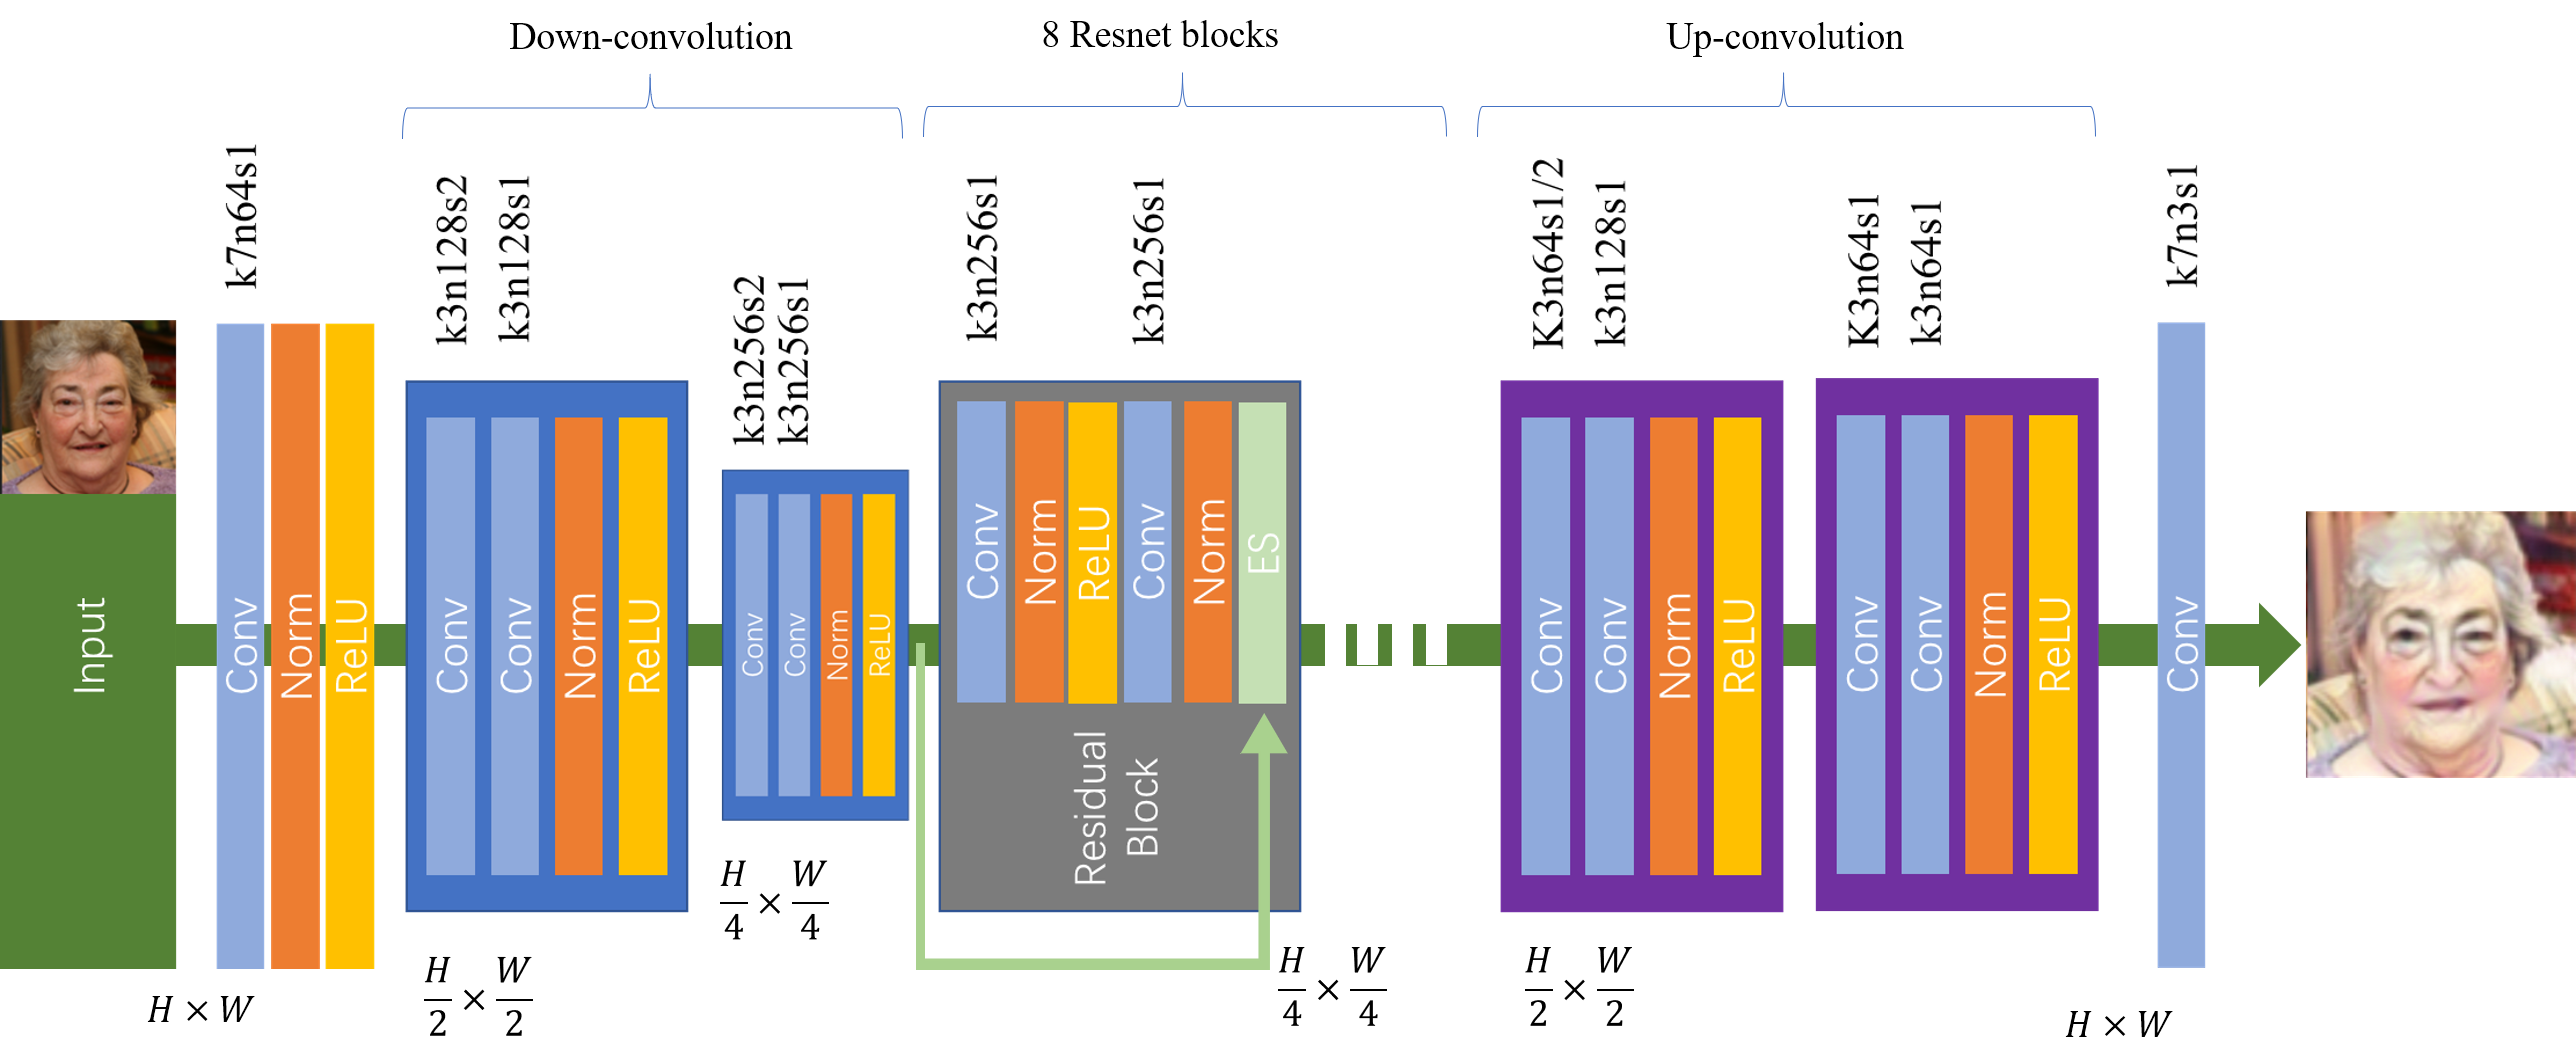
\includegraphics[width=.7\linewidth]{cartoongan-g}
      \caption{Generator of CartoonGAN}
   \end{subfigure}
   \begin{subfigure}{\linewidth}
      \centering
      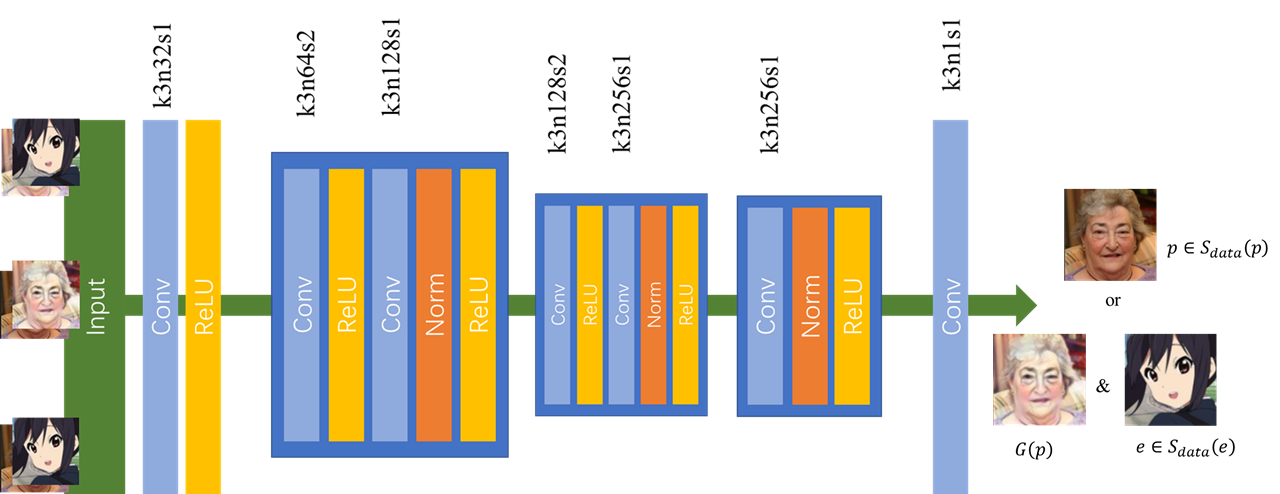
\includegraphics[width=.7\linewidth]{cartoongan-d}
      \caption{Discriminator of CartoonGAN}
   \end{subfigure}
   \caption{Architecture of CartoonGAN}
   \label{fig:cartoongan-arch}
\end{figure}

The datasets CartoonGAN uses are the same as the ones CycleGAN uses. But there
is one special preprocessing step, which creates another dataset based on Faces
(referred as $B$) through a process called edge promoting. We will refer this
generated dataset as $E$ hereinafter. During the process, first of all, edges
are detected, and then the pixels near the edges are convolved with Gaussian
kernel. This makes the edges in the pictures become smoother, in other words,
less sharper. The idea is that the picture of which edges are smooth should be
classified as real images, aka fake anime images, because cartoon images
generally have sharper edges. In addition, CartoonGAN uses a pretrained VGG19 as
feature extraction model for calculating content loss. We will refer it as
$VGG$.

We will refer the generator as $G$ and the discriminator as $D$. During the
training step of $D$, the BCE losses drive $D$ to classify $D(B)$ as real,
$D(G(A))$ and $D(E)$ as fake. During the training step of $G$, three losses are
added together:
\begin{itemize}[noitemsep, topsep=0pt]
   \item GAN loss: $D(G(A))$ should be classified as real.
   \item Content loss: $VGG(A)$ and $VGG(G(A))$ should be similar measured by L1
   loss, because the content of the source and generated images should be same.
   \item Style loss: $Gram(VGG(B))$ and $Gram(VGG(A))$ should be similar
   measured by L1 loss. Here $Gram$ means the Gram matrix. The idea is that the
   style of the target and generated images should be same.
\end{itemize}
Another notable thing is that generator goes through a pretrained process
minimizing the content loss.

In addition to the origin work, we also tried to add some loss functions to help
train the networks. These losses are:
\begin{itemize}[noitemsep, topsep=0pt]
   \item Face landmark loss: Give high priority to the key points on faces, so
   that the important features on faces can be preserved.
   This is inspired by \cite{wu2019landmark}.
   \item Grayscale loss and color loss: Proposed by someone, criticized and
   abandoned by me.
\end{itemize}

%------------------------------------------------------------------------
\section{Experiment}

\subsection{DCGAN}

\subsection{CycleGAN}

\subsection{CartoonGAN}

%------------------------------------------------------------------------
\section{Conclusion}

{\small
\bibliographystyle{ieee}
\bibliography{egbib}
}

\end{document}
